\documentclass[a4paper, table, 10pt]{article}
% Useful packages, sorted so packages of similar functionality are grouped together. Not all are essential to make the document work, however an effort was made to make this list as minimalistic as possible. Feel free to add your own!

% Essential for making this template work are graphicx, float, tabularx, tabu, tocbibind, titlesec, fancyhdr, xcolor and tikz. 

% Not essential, but you will have to debug the document a little bit when removing them are amsmath, amsthm, amssymb, amsfonts, caption, subcaption, appendix, enumitem, hyperref and cleveref.

% inputenc, lipsum, booktabs, geometry and microtype are not required, but nice to have.

\usepackage[utf8]{inputenc} % Allows the use of some special characters
\usepackage{amsmath, amsthm, amssymb, amsfonts} % Nicer mathematical typesetting
\usepackage[portuguese]{babel} % Portuguese language settings
% \usepackage[latin]{babel}
% \usepackage{lipsum} % Creates dummy text lorem ipsum to showcase typsetting 
\usepackage{setspace}
\usepackage{graphicx} % Allows the use of \begin{figure} and \includegraphics
\usepackage{float} % Useful for specifying the location of a figure ([H] for ex.)
\usepackage{caption} % Adds additional customization for (figure) captions
\usepackage{subcaption} % Needed to create sub-figures
\usepackage{tabularx} % Adds additional customization for tables
\usepackage{tabu} % Adds additional customization for tables
\usepackage{booktabs} % For generally nicer looking tables
\usepackage[nottoc,numbib]{tocbibind} % Automatically adds bibliography to ToC
\usepackage[margin = 2.54cm]{geometry} % Allows for custom (wider) margins
\usepackage{microtype} % Slightly loosens margin restrictions for nicer spacing  
\usepackage{titlesec} % Used to create custom section and subsection titles
\usepackage{titletoc} % Used to create a custom ToC
\usepackage{appendix} % Any chapter after \appendix is given a letter as index
\usepackage{fancyhdr} % Adds customization for headers and footers
\usepackage[shortlabels]{enumitem} % Adds additional customization for itemize. 
\usepackage{hyperref} % Allows links and makes references and the ToC clickable
\usepackage[noabbrev, capitalise]{cleveref} % Easier referencing using \cref{<label>} instead of \ref{}

\usepackage{xcolor} % Predefines additional colors and allows user defined colors

\usepackage{tikz} % Useful for drawing images, used for creating the frontpage
\usetikzlibrary{positioning} % Additional library for relative positioning 
\usetikzlibrary{calc} % Additional library for calculating within tikz

% Defines a command used by tikz to calculate some coordinates for the front-page
\makeatletter
\newcommand{\gettikzxy}[3]{%
  \tikz@scan@one@point\pgfutil@firstofone#1\relax
  \edef#2{\the\pgf@x}%
  \edef#3{\the\pgf@y}%
}
\makeatother



 % Loads in the preamble 
% Give your report a title
\newcommand\reporttitle{Kernel, Licenciamento e Segurança em Ambientes Open Source e Proprietários}

% Insert course code, name, quartile number and year (or any other subtitle)
\newcommand\reportsubtitle{
Sistemas Operativos Open Source (5116)
}

% Add your group number (for DBL) or any other text.
% \newcommand\groupnumber{
% \textbf{Group xx}
% }

% Insert authors and student numbers here
\newcommand\reportauthors{
Daniel Quaresma \\
Lucas Silvestre \\
João Correia \\
Vladimiro Bonaparte \\
}

% Add the name of your tutor (for DBL) or any other text.
\newcommand\grouptutor{
Formador: Nelson Alexandre Santos
}

% Date and location (default: current date and Eindhoven)
\newcommand\placeanddate{
\today
}

% Define Tue-red (color of the TU/e logo). Can be changed to drastically change the look of the template
\definecolor{Tue-red}{RGB}{50, 25, 180}

% All of the following code can be removed to be left with (close to) default LaTeX behaviour. 

% Sets up hyperlinks in the document to be colored
\hypersetup{
    colorlinks=true,
    linkcolor=Tue-red,
    urlcolor=Tue-red,
    citecolor = Tue-red
    }
\urlstyle{same} % Defines settings for link and reference formatting


% Change bullet style for level 1, 2 and 3 respectively for itemize
\renewcommand{\labelitemi}{\scriptsize\textcolor{Tue-red}{$\blacksquare$}}% level 1
\renewcommand{\labelitemii}{\scriptsize\textcolor{Tue-red}{$\square$}}% level 2
\renewcommand{\labelitemiii}{\textcolor{Tue-red}{$\circ$}}% level 3

% \renewcommand{\labelitemi}{\small\textcolor{Tue-red}{\ding{70}}} % level 1
% \renewcommand{\labelitemii}{\small\textcolor{Tue-red}{\ding{71}}}% level 2
% \renewcommand{\labelitemiii}{\tiny\textcolor{Tue-red}{\ding{71}}}% level 3

% Change bullet style for level 1, 2 and 3 respectively for enumerate
\renewcommand{\labelenumi}{\textbf{\textcolor{Tue-red}{\arabic*.}}}% level 1
\renewcommand{\labelenumii}{\textbf{\textcolor{Tue-red}{[\alph*]}}}% level 2
\renewcommand{\labelenumiii}{\textbf{\textcolor{Tue-red}{\roman*.}}}% level 3

% Have reference labels be linked to section (section 3 will have fig. 3.1 etc.)
\counterwithin{equation}{section} % For equations
\counterwithin{figure}{section} % For figures
\counterwithin{table}{section} % For tables

% Creates a beautiful header/footer
\pagestyle{fancy}
\lhead{
\includegraphics[height = 8pt]{Figures/0. General/atec_2.png}}
\rhead{\reporttitle}
\renewcommand{\footrulewidth}{0.4pt}
\cfoot{Página \thepage}

% Formats section, subsection and subsubsection titles respectively 
\titleformat{\section}{\sffamily\color{Tue-red}\Large\bfseries}{\thesection\enskip\color{gray}\textbar\enskip}{0cm}{} % Formats section titles

\titleformat{\subsection}{\sffamily\color{Tue-red}\large\bfseries}{\thesubsection\enskip\color{gray}\textbar\enskip}{0cm}{} % Formats subsection titles

\titleformat{\subsubsection}{\sffamily\color{Tue-red}\bfseries}{\thesubsubsection\enskip\color{gray}\textbar\enskip}{0cm}{} % Formats subsubsection titles

% Formats captions
\DeclareCaptionFont{Tue-red}{\color{Tue-red}}
\captionsetup{labelfont={Tue-red,bf}}

 % Changes font to mlmodern
\usepackage{mlmodern}

% Removes indent when starting a new paragraph
\setlength\parindent{0pt}

% Limits the ToC to sections and subsections (no subsubsec.)
\setcounter{tocdepth}{2}
 % Loads in user defined settings
\begin{document}

% Inserts the front page
\begin{titlepage}

\centering

\begin{tikzpicture}

\node[inner sep=0pt] (logo) at (0,0.6)
    {
\includegraphics[scale=0.04]{Figures/0. General/linux_penguin.png}};
{\setstretch{2.0}
\node[text width = 0.5\textwidth, yshift = 0.5cm, right = 1.25cm of logo](title){\sffamily\huge\reporttitle};
}   


\node[text width = 0.5\textwidth, yshift = 0.5cm, below = 0.5cm of title](subtitle){\sffamily\Large \reportsubtitle};

\gettikzxy{(subtitle.south)}{\sffamily\subtitlex}{\subtitley}
\gettikzxy{(title.north)}{\titlex}{\titley}
% \draw[line width=1mm, Tue-red]($(logo.east)!0.5!(title.west)$) +(0,\subtitley) -- +(0,\titley);

\end{tikzpicture}
\vspace{3cm}
% \sffamily\groupnumber

\begin{table}[H]
\centering
\sffamily
\large
\begin{tabu} to 2.8\linewidth {cc}
\textbf{Realizado por:}\\
% \hline
% \vspace{0.25cm}
\sffamily\reportauthors

\end{tabu}

\end{table}

\sffamily \grouptutor

\tikz[remember picture,overlay]\node[anchor=south,inner sep=0pt] at (current page.south) {\includegraphics[width=\paperwidth]{Figures/0. General/tue_2.png}};

\mbox{}
\vfill
\sffamily \Large \textcolor{white}{\placeanddate} \\



\end{titlepage}









\newpage

% Generates a ToC without page number
{\hypersetup{linkcolor=black} % Keeps the ToC black even with non-black linkcolor
\tableofcontents\thispagestyle{empty}}
\newpage

% Creates the introduction, starting page numbering
\section{Introdução} \label{section: Introducao}
\setstretch{1.15}
Nos últimos anos, o panorama da escolha de um Sistema Operativo (SO) tem sido marcado pela convivência entre soluções open source e proprietárias. Essa dualidade não apenas influencia a seleção de um usuário individual, mas também afeta os ambientes empresariais e governamentais.

O presente trabalho de investigação tem como objetivo explorar essa tendência, bem como destacar a importância do Kernel em um SO, abordar a questão da segurança em software open source e discutir os diferentes tipos de licenciamentos. Nesse contexto, é crucial compreender as vantagens e desvantagens ao optar por soluções de software open source ou proprietário. A decisão vai além das preferências individuais, pois impacta diretamente a eficiência, segurança e os custos associados.

Ao analisar essa dualidade, é essencial não apenas considerar as características técnicas dos SO, mas também avaliar as implicações legais, como licenciamento e conformidade.

A segurança da informação surge como um tema crucial nessa escolha. Muitos consideram os SO open source mais transparentes e suscetíveis a auditorias, porém potencialmente menos seguros em comparação aos SO proprietários. Essa preocupação com a segurança não se limita aos SO, mas se estende a todo tipo de software em geral.

O trabalho seguirá um índice estabelecido, abordando os seguintes tópicos: Introdução, Sistemas Operativos open source e proprietários, Kernel e sua importância, exemplos de utilização do Linux, licenciamento open source, segurança em software open source, aquisição e uso de software open source em ambientes empresariais, conclusão e referências.

\vspace{2cm}

\begin{figure}[H]
  \centering
  % width=\textwidth para imagem da largura do texto
  
\includegraphics[scale=0.15]{Figures/0. General/linux_penguin.png}
  \caption{Logotipo do GNU/Linux}
  \label{fig: style 1 imagem de teste}
\end{figure} \pagenumbering{arabic}
\newpage

% Capitulo 2
\section{Sistemas operativos \textit{open source} e proprietários} \label{section: sistemas operativos}
\subsection{Sistemas operativos \textit{open source} }
\textit{Open source} é um termo em inglês que significa "código aberto". Hoje, o \textit{open source} representa não apenas um movimento tecnológico, mas também uma filosofia de trabalho que transcende a produção de software. \cite{whatIsOpenSource}
\par \vspace{6pt}
Os sistemas operativos \textit{open source} são desenvolvidos colaborativamente por comunidades de programadores de todo o mundo. Algumas das suas características incluem: \cite{advantagesOfOpenSource}

\begin{itemize}

  \item \textbf{Código aberto}\\
  O código-fonte do sistema operativo é disponibilizado para o público, permitindo que qualquer pessoa estude, utilize, altere e distribua conforme os termos da licença de código aberto.

  \item \textbf{Transparência}\\
   A natureza transparente do desenvolvimento de código aberto possibilita que os utilizadores examinem o código para identificar e corrigir falhas de segurança, melhorar o desempenho e adicionar novos recursos.

  \item \textbf{Modelo de desenvolvimento colaborativo}\\
  Modelo de Desenvolvimento Colaborativo: O desenvolvimento de sistemas operativos \textit{open source} é caracterizado por uma abordagem colaborativa, na qual programadores voluntários contribuem com código, correções de bugs e melhorias de forma descentralizada.

  \item \textbf{Flexibilidade}\\
  Flexibilidade: Os sistemas operativos \textit{open source} são altamente personalizáveis, permitindo que os utilizadores adaptem o software às suas necessidades específicas. Isso é particularmente vantajoso em ambientes empresariais e de pesquisa.
\end{itemize}

\begin{figure}[H]
  \centering
  % width=\textwidth para imagem da largura do texto
  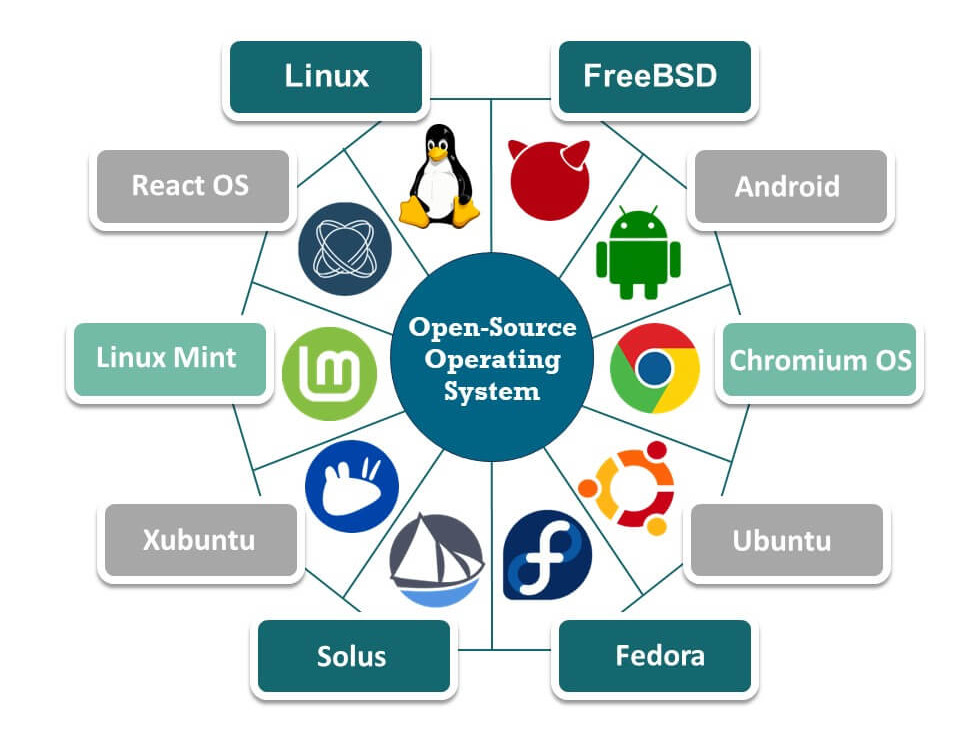
\includegraphics[scale=1.5]{Figures/0. General/sistemas_open_source.jpg}
  \caption{Tipos de sistemas \textit{open source}}
  \label{Tipos de sistemas open source}
\end{figure}

\newpage
\subsection{Sistemas operativos proprietários}
Enquanto os sistemas operativos open source promovem a colaboração, a transparência e a liberdade de personalização, os sistemas operativos proprietários oferecem conveniência, suporte profissional e uma experiência de utilizador refinada. \cite{advantagesOfProprietary}
\par \vspace{6pt}
A preferência por um tipo de SO sobre o outro muitas vezes reflete valores filosóficos, necessidades específicas de uso e considerações práticas, influenciando diretamente as decisões individuais e organizacionais de adoção de tecnologia.
\par \vspace{6pt}
Os sistemas operativos proprietários são desenvolvidos e mantidos por empresas que detêm os direitos de propriedade do software, as suas características são:

\begin{itemize}
  \item \textbf{Código Fechado}
  
      Os sistemas operativos proprietários são desenvolvidos por empresas que mantêm o código em sigilo, limitando o acesso dos utilizadores à sua inspeção e modificação.
  
  \item \textbf{Controle Centralizado}
  
      As empresas que desenvolvem sistemas operativos proprietários exercem um controlo centralizado sobre o desenvolvimento, distribuição e suporte do software, o que pode limitar a flexibilidade e a capacidade de personalização pelos utilizadores.
  
  \item \textbf{Suporte Profissional}
  
      Os sistemas operativos proprietários geralmente são acompanhados por serviços de suporte profissional oferecidos pelas empresas, o que pode ser vantajoso para utilizadores e organizações que valorizam a garantia de suporte técnico especializado.
  
  \item \textbf{Restrições de Licença}

      Os sistemas operativos proprietários geralmente são distribuídos com licenças restritivas que limitam o uso, distribuição e modificação do software pelos utilizadores. Essas restrições podem incluir proibições de redistribuição, limitações de uso em múltiplos dispositivos ou restrições de modificação do código fonte.
  
  \item \textbf{Ciclos de Atualização Controlados}
  
      As atualizações de sistemas operativos proprietários são frequentemente controladas e fornecidas pelas empresas desenvolvedoras de acordo com um cronograma predeterminado. Isso pode garantir uma maior consistência e estabilidade nas atualizações, mas pode também limitar a flexibilidade dos utilizadores em adotar novas funcionalidades ou correções de forma imediata.
\end{itemize}

\begin{figure}[H]
  \centering
  % width=\textwidth para imagem da largura do texto
  
\includegraphics[scale=0.2]{Figures/0. General/sistemas_proprietarios.jpg}
  \caption{Tipos de sistemas proprietários}
  \label{Tipos de sistemas proprietários}
\end{figure}

\newpage

% Capitulo 3
\section{\textit{Kernel}, qual a importância?} \label{section: kernel}

\subsection{O que é?}
O \textit{Kernel} é um componente fundamental de qualquer sistema operacional, sendo responsável pela gestão dos recursos de hardware e por fornecer uma interface entre o software e o hardware do computador. \cite{kernel}

\begin{figure}[H]
  \centering
  % width=\textwidth para imagem da largura do texto
  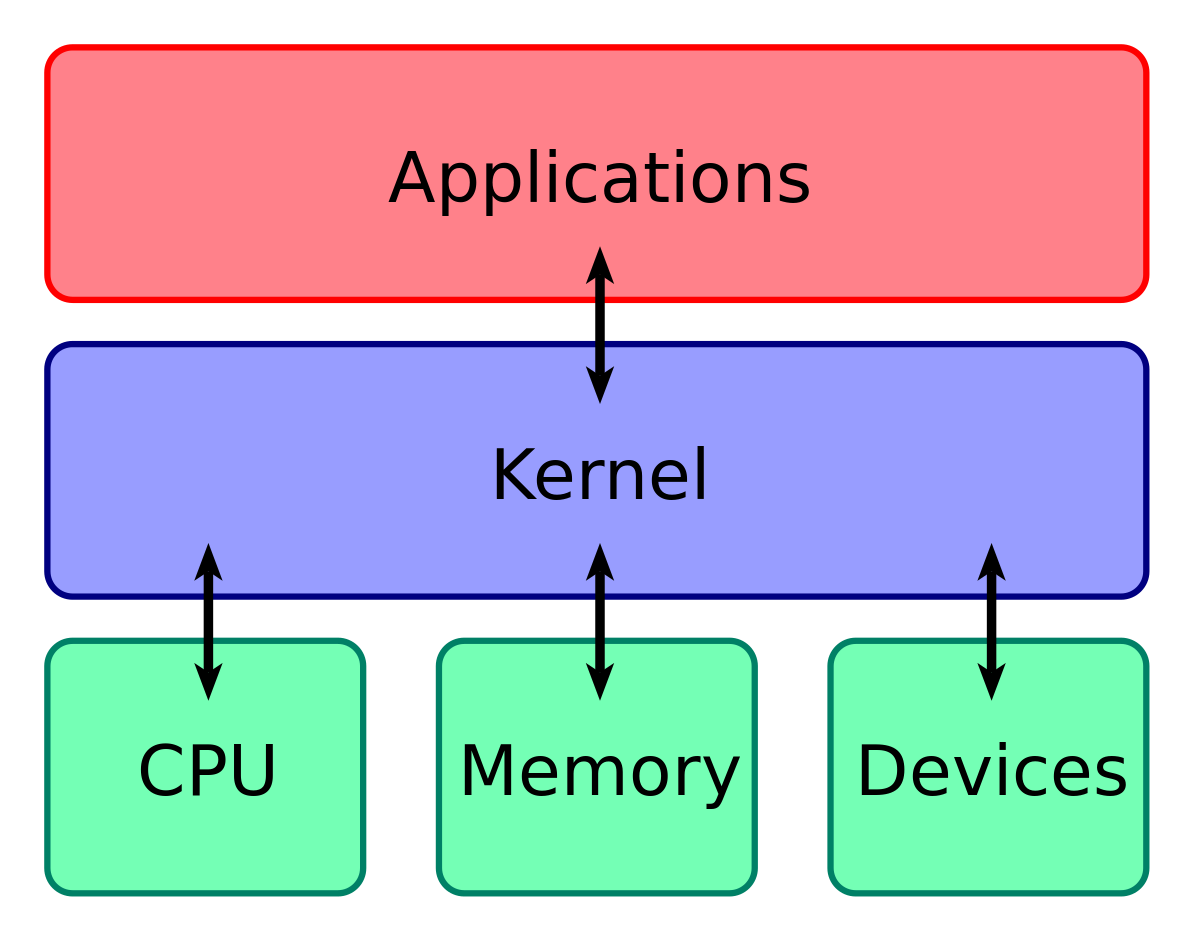
\includegraphics[scale=0.2]{Figures/0. General/kernel.png}
  \caption{Simplificação de como opera o \textit{Kernel}}
  \label{Simplificação da operação do Kernel}
\end{figure}

\subsection{Importância}
Algumas das responsabilidades do \textit{Kernel} são:

\begin{itemize}

  \item \textbf{Gestão de recursos}\\
  O \textit{Kernel} é responsável pela alocação e gestão dos recursos de hardware, garantindo que os processos em execução no sistema tenham acesso adequado à CPU, memória e dispositivos periféricos.

  \item \textbf{Abstração de hardware}\\
  O \textit{Kernel} fornece uma camada de abstração entre o software e o hardware, permitindo que os desenvolvedores de aplicativos escrevam código independente de plataforma. Isso facilita o desenvolvimento de software portátil e compatível com diferentes sistemas operativos.

  \item \textbf{Execução de tarefas do sistema}\\
  O \textit{Kernel} é responsável pela execução de tarefas essenciais do sistema, como o agendamento de processos, gestão de memória virtual, gestão de interrupções e controlo de dispositivos de entrada e saída.

  \item \textbf{Segurança e proteção}\\
  O \textit{Kernel} implementa mecanismos de segurança e proteção para garantir a integridade e a segurança do sistema e dos dados dos utilizadores. Controla o acesso aos recursos do sistema e impede que processos maliciosos comprometam a estabilidade do sistema.

  \item \textbf{Desempenho e eficiência}\\
  Um \textit{Kernel} eficiente é essencial para o desempenho e a eficiência do sistema operativo como um todo. Deve ser otimizado para minimizar o tempo de resposta, maximizar a utilização dos recursos de hardware e garantir uma experiência de utilizador fluída.
\end{itemize}

\newpage

% Capitulo 4
\section{Linux e exemplos de utilização} \label{section: linux e exemplos}

\subsection{História}
O \textbf{GNU/Linux} é um sistema operativo \textit{open source}, criado por \textbf{Linus Torvalds} em 1991 após a sua exposição inicial a sistemas \textbf{Unix} enquanto estudante de informática na Universidade de Helsínquia, na Finlândia.
\par \vspace{6pt}
O nome \textbf{Linux} é uma combinação do primeiro nome de seu criador, \textbf{Linus}, e do sistema operativo \textbf{Unix}, que serviu de inspiração para os seus projetos. Na altura, a maioria dos sistemas operativos era proprietária e cara, levando Linus a decidir criar um sistema operativo que estivesse disponível gratuitamente para qualquer pessoa. \cite{linuxHistory}
\par \vspace{6pt}
O Projeto \textbf{GNU}, liderado por \textbf{Richard Stallman} desde 1983, é fundamental para a história do Linux. Ao oferecer um conjunto completo de ferramentas e utilitários de software livre, o \textbf{GNU} forneceu a base essencial para várias distribuições Linux. Além disso, o \textbf{GNU} também contribuiu para a nomenclatura oficial, dando origem ao nome \textbf{GNU/Linux}. Essa colaboração entre o \textbf{GNU} e o kernel \textbf{Linux} resultou em sistemas operativos mais robustos e na capacidade de manter o GNU/Linux completamente livre. \cite{gnuHistory}
\par \vspace{6pt}
As primeiras versões do GNU/Linux eram principalmente utilizadas por entusiastas da tecnologia e desenvolvedores de software. Com o passar do tempo, a sua popularidade cresceu rapidamente, levando à sua adoção em uma ampla gama de ambientes.
\par \vspace{6pt}
O GNU/Linux é reconhecido como um dos sistemas operativos mais estáveis, seguros e confiáveis, sendo amplamente adotado em \textbf{servidores}, \textbf{supercomputadores} e \textbf{ambientes empresariais}. Com o crescimento de sua popularidade e o contínuo desenvolvimento pela comunidade, hoje, algumas das principais distribuições GNU/Linux incluem o \textbf{Ubuntu, Fedora, Arch, Red Hat, Debian, Mint} e \textbf{Manjaro}.

\par \vspace{13pt}

\begin{figure}[H]
    \centering
    % width=\textwidth para imagem da largura do texto
    
\includegraphics[scale=2.8]{Figures/0. General/linux_distros.png}
    \caption{Tipos de distribuições ou "distros" de linux}
    \label{Distros de linux}
\end{figure}

\newpage
\subsection{Presença em diversos ambientes}
O GNU/Linux está presente em uma ampla variedade de ambientes, incluindo: \cite{diverseUsage}
\begin{itemize}

    \item \textbf{Servidores e data centers}\\
    O GNU/Linux é amplamente reconhecido pelo seu domínio no mercado de servidores e centros de dados, destacando-se pela sua estabilidade e confiabilidade. É frequentemente utilizado para operar \textbf{redes de dados} e \textbf{data centers}.

    Muitos dos equipamentos constituintes dos servidores e data centers, tais como os \textbf{routers}, funcionam com versões personalizadas e simplificadas do sistema operativo GNU/Linux.

    \item \textbf{Supercomputadores}\\
    A capacidade do GNU/Linux para escalar eficientemente até milhares de núcleos de processamento, aliada à sua flexibilidade para otimização em tarefas de alto desempenho, são características essenciais para o seu uso em supercomputadores. 
    
    Na verdade, o GNU/Linux é o sistema operativo preferido para a maioria dos supercomputadores, evidenciando a sua eficiência em ambientes de computação intensiva.
    
    \item \textbf{Dispositivos IoT}\\
    No âmbito da \textbf{Internet das Coisas (IoT)}, o GNU/Linux destaca-se devido ao seu tamanho compacto e à sua capacidade de adaptação para se adequar a hardware específico. Desde \textbf{eletrodomésticos inteligentes} até sistemas avançados de \textbf{controlo industrial} e \textbf{veículos autónomos}, o GNU/Linux serve como uma base fiável para uma variedade de dispositivos inovadores.

    \item \textbf{Desktops e uso diário}\\
    Embora seja menos popular que o \textbf{Windows} ou o \textbf{MacOS} em desktops, o GNU/Linux tem observado um aumento constante na sua aceitação por parte dos utilizadores. Esta tendência deve-se à sua crescente biblioteca de programas de software baseados em GNU/Linux e a um foco contínuo na expansão da oferta de interfaces de utilizador mais amigáveis para desktop. Além disso, o sistema operativo GNU/Linux serve como a base de outros sistemas operativos amplamente utilizados no nosso quotidiano, como o \textbf{Android} e o \textbf{Chrome OS}.

    \item \textbf{Educação e governo}\\
    O GNU/Linux é altamente valorizado por instituições educativas e governamentais devido ao seu baixo custo e à sua capacidade de personalização. Em todo o mundo, vários governos têm implementado extensivamente o GNU/Linux nas operações governamentais e nos sistemas educacionais, aproveitando essas vantagens.
\end{itemize}

\par \vspace{6pt}

\begin{figure}[H]
    \centering
    % width=\textwidth para imagem da largura do texto
    
\includegraphics[scale=0.4]{Figures/0. General/super_computer.jpg}
    \caption{Supercomputador da IBM a correr Linux}
    \label{Supercomputador da IBM a correr Linux}
\end{figure}
\newpage

% Capitulo 5
\section{Licenciamento open source} \label{section: licenciamento}
% \lipsum[1-8]
texto
\newpage

% Capitulo 6
\section{Segurança em sistemas operativos \textit{open source}} \label{section: segurança}
\subsection{Importância da segurança}
O software de \textit{open source} tornou-se amplamente utilizado nos últimos anos devido à sua natureza colaborativa e pública, o que o torna conveniente tanto para os desenvolvedores como para os atores maliciosos. 
\par \vspace{6pt}
Quando adversários descobrem que uma aplicação está exposta a uma vulnerabilidade conhecida publicamente, podem atacar qualquer aplicação desenvolvida utilizando esse código de \textit{open source}. Casos como as vulnerabilidades do \textbf{Log4j} e do \textbf{Apache Struts} demonstram que isso representa um risco real e, por vezes, grave para as organizações. \cite{openSourceSecurity}
\subsection{Principais riscos}
A maioria das aplicações nativas em \textit{cloud} depende de componentes de \textit{open source}. Contudo, devido à ausência de responsabilidade pela sua manutenção ou segurança, o software de \textit{open source} apresenta diversos riscos, tais como:
\begin{itemize}

  \item \textbf{Vulnerabilidades em dependências}\\
  Essas vulnerabilidades podem ser tanto conhecidas quanto desconhecidas. As conhecidas incluem aquelas que receberam um número de identificação de vulnerabilidade comum \textbf{(CVE)}, aquelas divulgadas na Internet, aquelas presentes em bases de dados públicas de vulnerabilidades, e aquelas dentro de bases de dados privadas. Em geral, quanto mais conhecida for uma vulnerabilidade, mais urgente é a necessidade de solucioná-la.
  \par \vspace{6pt}
  Além de rastrear vulnerabilidades, é essencial acompanhar todas as dependências de \textit{open source} dentro de uma aplicação. As dependências transitivas, onde uma dependência depende de outras, são especialmente preocupantes, pois são menos visíveis para ferramentas de segurança e auditorias. Portanto, é útil utilizar ferramentas ou processos que possam identificar e auditar todas as dependências em uma aplicação.
  \item \textbf{Riscos de conformidade com licenças}\\
  Os desenvolvedores precisam compreender cada tipo de licença de software nos pacotes de \textit{open source} que utilizam, para poderem empregar o código de forma compatível. Isso requer conhecimento das estipulações de licenciamento e sua aplicação ao longo dos projetos. 
  \par \vspace{6pt}
  Para garantir o cumprimento das licenças de \textit{open source}, as organizações precisam ter uma visão aprofundada de como os componentes de \textit{open source} estão a ser utilizados. Também é importante monitorar continuamente as licenças, pois o proprietário dos direitos autorais pode alterar a licença de uma biblioteca.
  \item \textbf{Pacotes não mantidos}\\
  Os pacotes de \textit{open source} são geralmente mantidos por um único desenvolvedor ou por uma pequena equipa, quando são mantidos. Os desenvolvedores de projetos de \textit{open source} da comunidade não têm obrigação de manter o software, e ele é disponibilizado "como está". 
  \par \vspace{6pt}
  Cabe aos utilizadores dedicar tempo e recursos para garantir que o código seja seguro. Felizmente, existem ferramentas úteis que podem simplificar este processo analisar pacotes de acordo com o nível de manutenção, envolvimento da comunidade, postura de segurança e popularidade, auxiliando na avaliação da saúde dos pacotes de \textit{open source} utilizados. 
\end{itemize}
\newpage

% Capitulo 7
\section{Software \textit{open source} em ambientes empresários} \label{section: aquisição}
\subsection{Porquê?}
Software de \textit{open source} ou proprietário? As empresas enfrentam esta questão fundamental quando se trata de escolher aplicações críticas para o seu negócio. 
\par \vspace{6pt}
A decisão sobre o software adequado tem implicações a longo prazo e, portanto, deve ser considerada cuidadosamente. as empresas continuam a aumentar o seu uso de software de \textit{open source} nos últimos anos. Mesmo que muitas empresas não estejam cientes, o software de \textit{open source} já está presente em mais de 90\% das empresas em apoio à sua infraestrutura de TI. \cite{whyOpenSource}

\begin{figure}[H]
  \centering
  % width=\textwidth para imagem da largura do texto
  
\includegraphics[scale=0.6]{Figures/0. General/enterprise_open_source.jpg}
  \caption{Empresas cada vez aderem mais a \textit{open source}}
  \label{Empresas cada vez aderem mais a open source}
\end{figure}

\subsection{Beneficios}
Algumas das principais razões que as empresas dão para a utilização de software de \textit{open source}: \cite{stateOfEnterpriseOpenSource}

\begin{itemize}
  \item \textbf{Familiaridade}\\
  A Compreensão por parte dos desenvolvedores da colaboração com comunidades, contribuições para projetos, entendimento de licenças e gestão de dependências.
  \item \textbf{Apoio a comunidades}\\
  O sucesso do software \textit{open source} depende de comunidades saudáveis. Empresas podem contribuir com recursos, financiamento e feedback, fortalecendo tanto os projetos quanto a comunidade de \textit{open source}.
  \item \textbf{Capacidade de influenciar o desenvolvimento dos recursos necessários}\\
  Software \textit{open source} oferece transparência e adaptação às necessidades específicas. As empresas podem influenciar ativamente o desenvolvimento de recursos, seja contribuindo com código ou fornecendo feedback valioso.
  \item \textbf{Eficiência ao Lidar com Desafios Técnicos}\\
  Acesso a uma vasta comunidade de especialistas permite solucionar desafios técnicos de forma rápida e eficaz. Fóruns online e grupos de discussão facilitam a obtenção de suporte.
\end{itemize}
\newpage

% Capitulo 8
\section{Conclusão} \label{section: introdução}
Uma análise detalhada dos sistemas operativos \textit{open source} e proprietários revela uma série de considerações importantes para empresas que queiram adotá-los.
\par \vspace{6pt}
A importância do \textit{kernel} como o núcleo de qualquer sistema operativo é inegável, influenciando diretamente o desempenho, a estabilidade e a segurança do sistema. O \textit{kernel} Linux, em particular, destaca-se como um exemplo proeminente, oferecendo uma vasta gama de utilizações em diferentes contextos.
\par \vspace{6pt}
O licenciamento \textit{open source} apresenta tanto oportunidades quanto desafios, oferecendo liberdade e flexibilidade aos utilizadores, mas exigindo uma compreensão clara das obrigações legais associadas. No que diz respeito à segurança, embora os sistemas operativos \textit{open source} geralmente desfrutem de uma reputação de segurança robusta, é crucial adotar práticas de segurança adequadas e estar ciente das vulnerabilidades potenciais.
\par \vspace{6pt}
Para as empresas, a adoção de software \textit{open source} em ambientes empresariais pode oferecer uma série de vantagens, incluindo custos reduzidos, maior flexibilidade e acesso a uma vasta comunidade de desenvolvedores em troca de menos suporte profissional e estabilidade.
\par \vspace{6pt}
Em última análise, a escolha entre sistemas operativos \textit{open source} e proprietários é uma decisão estratégica que deve ser cuidadosamente ponderada, levando em consideração as necessidades específicas e os objetivos de negócios de cada empresa.
\par \vspace{6pt}
Ao compreender os diferentes aspectos envolvidos e considerando as implicações a longo prazo, as empresas devem fazer um estudo prévio, fazer um balanço entre os pontos positivos e negativos e tomar uma decisão informada sobre o tipo de sistemas a usar.
\par\vspace{24pt}

Todos os elementos do grupo participaram e alteraram o trabalho inteiro, mas o levantamento de informação de cada capítulo foi feito da seguinte maneira:
\begin{itemize}
\item \textbf{Daniel Quaresma}: Introdução e conclusão.
\item \textbf{Vladimiro Bonaparte}: Capítulo 2 e 3.
\item \textbf{Lucas Silvestre}: Capítulo 4 e 5.
\item \textbf{João Correia}: Capítulo 6 e 7.
\end{itemize}

\newpage

% contains inspiration for formatting tables, images, text citations etc.
% \section{This is a section} \pagenumbering{roman}
\subsection{This is a subsection}

\subsubsection{This is a subsubsection}
This section contains some templates that can be used to create a uniform style within the document. It also shows of the overall formatting of the template, created using the predefined styles from the \texttt{settings.tex} file.

\subsection{General formatting}
Bullet lists are also changed globally, for a maximum of 3 levels:

\begin{itemize}
    \item Item 1
    \item Item 2
    \begin{itemize}
        \item subitem 1
        \begin{itemize}
            \item subsubitem 1
            \item subsubitem 2
        \end{itemize}
    \end{itemize}
    \item Item 3
\end{itemize}

Similarly numbered lists are also changed document wide:

\begin{enumerate}
    \item Item 1
    \item Item 2
    \begin{enumerate}
        \item subitem 1
        \begin{enumerate}
            \item subsubitem 1
            \item subsubitem 2
        \end{enumerate}
    \end{enumerate}
    \item Item 3
\end{enumerate}

\newpage

\subsection{Tables and figures}
The following table, \cref{table: style 1}, shows a possible format for tables in this document. Alternatively, one can also use the black and white version of this, shown in \cref{table: style 2}. Note that caption labels are in the format \textbf{\textcolor{color_scheme}{Table x.y:} }
\begin{table}[ht]
\rowcolors{2}{color_scheme!10}{white}
\centering
\caption{A table without vertical lines.}
\begin{tabular}[t]{ccccc}
\toprule
\color{color_scheme}\textbf{Column 1}&\color{color_scheme}\textbf{Column 2}&\color{color_scheme}\textbf{Column 3}&\color{color_scheme}\textbf{Column 4}&\color{color_scheme}\textbf{Column 5}\\
\midrule
Entry 1&1&2&3&4\\
Entry 2&1&2&3&4\\
Entry 3&1&2&3&4\\
Entry 4&1&2&3&4\\
\bottomrule
\end{tabular}
\label{table: style 1}
\end{table}

\begin{table}[ht]
\rowcolors{2}{gray!10}{white}
\centering
\caption{A table without vertical lines.}
\begin{tabular}[t]{ccccc}
\toprule
\textbf{Column 1}&\textbf{Column 2}&\textbf{Column 3}&\textbf{Column 4}&\textbf{Column 5}\\
\midrule
Entry 1&1&2&3&4\\
Entry 2&1&2&3&4\\
Entry 3&1&2&3&4\\
Entry 4&1&2&3&4\\
\bottomrule
\end{tabular}
\label{table: style 2}
\end{table}

% For normal, single image figures, the standard \texttt{\textbackslash begin\{figure\}} environment can be used. For multi-image figures, one could use either the \texttt{\textbackslash begin\{subfigure\}} environment to get a main caption with 3 subcaptions like \cref{fig: three images} or the \texttt{\textbackslash begin\{minipage\}} environment to get 3 independent captions like \cref{fig: style 2 image a} - \ref{fig: style 2 image c}

\begin{figure}[H]
     \centering
     \begin{subfigure}[b]{0.3\textwidth}
         \centering
         \includegraphics[width=\textwidth]{example-image-a}
         \caption{image a}
         \label{fig: style 1 image a}
     \end{subfigure}
     \hfill
     \begin{subfigure}[b]{0.3\textwidth}
         \centering
         \includegraphics[width=\textwidth]{example-image-b}
         \caption{image b}
         \label{fig: style 1 image b}
     \end{subfigure}
     \hfill
     \begin{subfigure}[b]{0.3\textwidth}
         \centering
         \includegraphics[width=\textwidth]{example-image-c}
         \caption{image c}
         \label{fig: style 1 image c}
     \end{subfigure}
        \caption{Three images}
        \label{fig: three images}
\end{figure}

\begin{figure}[H]
\centering
\begin{minipage}{0.3\textwidth}
  \centering
  \includegraphics[width=\textwidth]{example-image-a}
  \captionof{figure}{image a}
  \label{fig: style 2 image a}
\end{minipage}
\hfill
\begin{minipage}{0.3\textwidth}
  \centering
  \includegraphics[width=\textwidth]{example-image-b}
  \captionof{figure}{image b}
  \label{fig: style 2 image b}
\end{minipage}
\hfill
\begin{minipage}{0.3\textwidth}
  \centering
  \includegraphics[width=\textwidth]{example-image-c}
  \captionof{figure}{image c}
  \label{fig: style 2 image c}
\end{minipage}
\end{figure} % Feel free to remove / comment out
% \newpage

% Generates a list of symbols table
% \section*{list of symbols} \label{section: symbols}

\begin{table}[ht]
\rowcolors{2}{gray!10}{white}
\centering
\caption{list of symbols}
\begin{tabular}[t]
{m{0.1\textwidth}m{0.25\textwidth}m{0.25\textwidth}m{0.2\textwidth}}
\toprule
\textbf{Symbol}&\textbf{dimension}&\textbf{Unit}&\textbf{Unit abbreviation}\\
\midrule
1&2&3&4\\
1&2&3&4\\
1&2&3&4\\
1&2&3&4\\
\bottomrule
\end{tabular}
\end{table}
% \newpage


% Creates references using the Biblatex 
\bibliographystyle{unsrt}
\bibliography{General/References.bib}
\newpage

\appendix % Any section after this command will have a letter as an index

% Adds an appendix entry
% \section{Apêndice A - Referências} \label{section: appendix A title}
texto
% \newpage

\end{document}
